\documentclass[9pt]{beamer}
\usepackage{styles/mypreamble}
%~~~~~~~~~~~~~~~~~~~~~~~~~~~~~~~~~~~~~~~~~~~~~~~~~~~~~~~~~~~~~~~~~~~~~~~~~~~~~~
\title{Алгоритмы машинного обучения}
\subtitle{Лекция 8. Обучение с учителем. Метрики качества.}
\author{Владимир Кукушкин}
\institute{СПбГЭУ - 2020}
\date{\today}
%~~~~~~~~~~~~~~~~~~~~~~~~~~~~~~~~~~~~~~~~~~~~~~~~~~~~~~~~~~~~~~~~~~~~~~~~~~~~~~

\begin{document}

\titlepage

\section{Постановка задачи supervised learning}

\begin{frame}{Supervised learning}
\begin{itemize}
    \item Supervised learning -- обучение с учителем.
    \item Предполагаем, что существует зависимость $f(x) = y$, где $x\in \sf{X}$ – некоторый объект, $y\in \sf{Y}$ – некоторый результат наблюдения за объектом.
\end{itemize}
\end{frame}

\begin{frame}{Supervised learning}
\begin{itemize}
    \item Даны матрица "объект-признак"\; $X$ и таргетная переменная $Y$:
$$X = \begin{pmatrix}x_{11}&x_{21}&\ldots&x_{1p}\\x_{21}&x_{22}&\ldots&x_{2p}\\\ldots&\ldots&\ddots&\ldots\\x_{N1}&x_{N2}&\ldots&x_{Np}\\\end{pmatrix},\;\;
y = \begin{pmatrix}y_1\\ \vdots \\ y_N \end{pmatrix}
$$
    \item Предполагаем, что есть зависимость $f(x) = y$ и хотим её восстановить: то есть найти такую модель $\hat a$, чтобы $\hat a(x) \approx y$.
\end{itemize}
\end{frame}

\begin{frame}{Общая схема решения задач supervised learning}
    \begin{itemize}
        \item Определяем функцию ошибки $L(a, X)$.
        \item Определяем семейство моделей $A = \{a(x, \theta)\; : \sf{X} \rightarrow \sf{Y} \; | \; \theta \in \Theta\}$.
        \item Разбиваем датасет на два множества $X = X_{train} \sqcup X_{test}$.
        \item Обучаем модель на $X_{train}$. Находим $\hat \theta = \underset{\Theta}{\mathrm{arg\;min}}\;L(\theta, X_{train})$.
        \item Проверяем качество модели на $X_{test}$. Вычисляем $L(\hat a, X_{test})$.
    \end{itemize}
\end{frame}

\begin{frame}{Пример}
\begin{itemize}
    \item Модель линейной регрессии: ищем решение в виде
    $$a(x_i) = \beta_1 x_{i1} + \ldots + \beta_p {x_{ip}} + \beta_0.$$
    \item $\Theta = \{\beta_0, \beta_1, \ldots, \beta_p\} = \mathbb{R}^{p+1}$ -- множество параметров модели.
    \item $L(x) = \frac{1}{N}\sum\limits_{i=1}^N(a(x_i) - y_i)^2$ -- среднеквадратичная ошибка.
    \item Тогда решением задачи будут параметры $\hat\beta_0, \hat\beta_1, \ldots, \hat\beta_p$, минимизирующие функционал ошибок:
    $$\hat\theta = (\hat\beta_0, \hat\beta_1, \ldots, \hat\beta_p) = \underset{\beta_0, \beta_1,\ldots, \beta_p}{\arg\min}\;  \frac{1}{N}\sum\limits_{i=1}^N( (\beta_1 x_{i1}  + \ldots + \beta_p x_{ip} + \beta_0) - y_i)^2.$$
\end{itemize}
\end{frame}


\begin{frame}{Типы задач}
Пусть $y_i \in \sf{Y}$ -- множество допустимых значений $y$.
\begin{itemize}
    \item Задача классификации.
    \begin{itemize}
        \item Бинарная классификация: $\sf{Y} = \{0, 1\}$.
        \item Мультиклассовая классификация: $\sf{Y} = \{1, \ldots, M\}$.
    \end{itemize}
    \item Задача регрессии: $\sf{Y} = \mathbb{R}$.
    \item Задача ранжирования: $\sf{Y} = \{1, \ldots, N\}$.
\end{itemize}
    
\end{frame}

\section{Функционалы качества}

\begin{frame}{Функционалы качества}
\begin{itemize}
    \item Функционалы качества выбираются в зависимости от типа задачи и её индивидуальных особенностей.
\end{itemize}
\end{frame}

\subsection{Бинарная классификация}

\begin{frame}{Точность (accuracy)}
\begin{itemize}
    \item \textbf{Точность} (a.k.a. \textbf{accuracy}): $L(a, X) = \frac{\#\{\hat y_i \neq y_i\}}{N}$.
    \item Плюсы: простой, понятен любому менеджеру.
    \item Минусы: работает только в случае сбалансированной выборки (Доли 0 и 1 в $y$ различаются не сильно).
\end{itemize}

Пример.\newline
Пусть мы решаем антифрод-задачу. В репрезентативной выборке пользователей доля мошенников будет низкой. Пусть она равна 1\%. Тогда точность классификатора, всегда возвращающего 0, будет равна 99\%.
\end{frame}

\begin{frame}{Матрица ошибок}
    \begin{itemize}
        \item Сравним результаты предсказаний с истинными значениями и запишем количества различных четырёх исходов в \textbf{матрицу ошибок}:
    $$
    \begin{tabular}{|c|c|c|}
    \hline
         & $y = 0$ & $y = 1$\\ \hline 
    $\hat y = 0$ & True Negative (TN) & False Negative (FN)  \\ \hline 
    $\hat y = 1$ & False Positive (FP) & True Positive (TP)  \\ \hline 
    \end{tabular}
    $$
    \item \textbf{Точность} (a.k.a. \textbf{precision}): $\frac{TP}{TP + FP}$ -- количество правильно предсказанных единичек среди всех \textit{предсказанных} единичек.
    \item \textbf{Полнота} (a.k.a. \textbf{recall}): $\frac{TP}{TP + FN}$ -- количество правильно предсказанных единичек среди всех \textit{истинных} единичек.
    \item Точность, которая accuracy, запишется как $\frac{TN + TP}{TN + FP + FN + FP}$.
    \end{itemize}
У dummy-классификатора (на 100 точках) полнота 0 и точность NA: 
    $$
    \begin{tabular}{|c|c|c|}
    \hline
         & $y = 0$ & $y = 1$\\ \hline 
    $\hat y = 0$ & 99 & 1  \\ \hline 
    $\hat y = 1$ & 0 & 0 \\ \hline 
    \end{tabular}
    $$
Приведите примеры задач, в которых больше важна точность/полнота.
\end{frame}

\begin{frame}{Другие метрики на матрице ошибок}
    $$
    \begin{tabular}{|c|c|c|}
    \hline
         & $y = 0$ & $y = 1$\\ \hline 
    $\hat y = 0$ & True Negative (TN) & False Negative (FN)  \\ \hline 
    $\hat y = 1$ & False Positive (FP) & True Positive (TP)  \\ \hline 
    \end{tabular}
    $$
    \begin{itemize}
        \item $\text{TPR (True Positive Rate, a.k.a. sensitivity, recall)} = \frac{TP}{TP + FN} = 1 - FNR$
        \item $\text{TNR (True Negative Rate, a.k.a. specificity)} = \frac{TN}{TN + FP} = 1 - FPR$
        \item $\text{FPR (False Positive Rate)} = \frac{FP}{FP + TN}$
        \item $\text{FNR (False Negative Rate)} = \frac{FN}{FN + TP}$
    \end{itemize}
\begin{itemize}
    \item Обычно используют пары метрик: precision + recall, sensitivity + specificity, TPR + FPR.
    \item Пара метрик хорошо, но хочется получить какую-то одну чиселку для принятия решения.
\end{itemize}
\end{frame}

\begin{frame}{ROC AUC}
\begin{itemize}
    \item Практически все бинарные классификаторы считают некоторый скор, который сравнивается с пороговым значением, после чего принимается решение, к какому из классов -- 0 или 1 -- принадлежит объект.
    \item Пройдёмся сеткой по возможным пороговым значениям, посчитаем в каждой точке TPR, FPR и отобразим их на графике. Получится т.н. ROC-кривая (Receiver Operating Characteristic curve).
    \item Чем выпуклее кривая, тем лучше. Диагональ соответствует рандомному классификатору (выдаёт одинаковое количество TP и FP).
    \item Как измерить выпуклость? Посчитать площадь под кривой. Это и есть AUC (Area Under Curve).
    \item Можно считать площадь под precision+recall кривой, но TPR+FPR для этих целей применяется чаще.
\end{itemize}
\end{frame}

\framedgraphic{ROC AUC. Пример.}{img/roc_auc.png}
\begin{frame}{F-мера}
    \begin{itemize}
        \item Ещё одним из вариантов свести две чиселки в одну является $F_1$-мера (среднее гармоническое):
        $$F_1 = 2 \frac{\text{Precision}\cdot \text{Recall}}{\text{Precision} + \text{Recall}}.$$
        \item Часто в конкретных задачах уделяется особое внимание отдельно точности или полноте. Тогда можно регулировать эту важность с помощью веса $\beta > 0$:
        $$F_\beta = (\beta^2 + 1) \frac{\text{Precision}\cdot \text{Recall}}{\beta^2 \cdot \text{Precision} + \text{Recall}}.$$
        При $0 < \beta < 1$ предпочтение отдаётся точности, при $\beta > 1$ -- полноте.
    \end{itemize}
\end{frame}

\begin{frame}{Logistic Loss}
\begin{itemize}
    \item Пусть $a(x_i) = \hat p_i$ -- вероятность принадлежности классу 1. Тогда logistic loss (логлосс) определяется как:
    $$L(a, X) = - \frac{1}{N}\sum_{i=1}^N\left(y_i \log(\hat y_i) + (1 - y_i)\log(1 - \hat y_i)\right).$$
    \item Подробнее о природе этой функции поговорим на лекции про логистическую регрессию.
    \item Заметим, что штраф за высокую уверенность классификатора в неверном ответе очень высок.
    \item В бизнес-требованиях эта метрика встречается редко, однако в целом в data science она достаточно распространена.
\end{itemize}
\begin{center}
    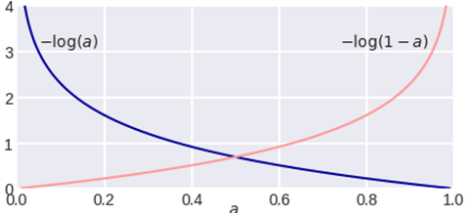
\includegraphics[height=0.3\textheight]{img/log_loss.png}    
\end{center}
\end{frame}

\begin{frame}{Мультиклассовая классификация}
\begin{itemize}
    \item ROC-AUC работает только для бинарной классификации.
    \item Будем считать точность и полноту для каждого класса классификации.
    $$
    \begin{tabular}{|c|c|c|c|}
    \hline
         & $y = 1$ & $\cdots$ & $y = M$\\ \hline 
    $\hat y = 1$ & $A_{11}$ & $\cdots$ & $A_{1M}$  \\ \hline 
    $\cdots$ & $\cdots$ & $\cdots$ & $\cdots$  \\ \hline 
    $\hat y = M$ & $A_{M1}$ & $\cdots$ & $A_{MM}$  \\ \hline 
    \end{tabular}
    $$
    \item $\text{Precision}_k = \frac{A_{kk}}{\sum\limits_{i=1}^M A_{ki}}$ (делим на сумму по строке).
    \item $\text{Recall}_k = \frac{A_{kk}}{\sum\limits_{i=1}^M A_{ik}}$ (делим на сумму по колонке).
    \item Итоговой точностью/полнотой классификатора можно считать среднее арифметическое точности и полноты по всем классам (macro-averaging подход).
    \item $\text{Logloss} = -\frac{1}{N}\sum\limits_{i=1}^N\sum\limits_{j=1}^M y_{ij}\log(a_{ij})$, где $y_{ij}=\mathds{1}(y_{i} = j)$, $a_{ij}=P(y_i = j)$.
\end{itemize}
\end{frame}

\subsection{Регрессия}

\begin{frame}{Основные метрики качества для регрессии}
\begin{itemize}
    \item $\text{MSE} = \frac{1}{N}\sum\limits_{i=1}^N (y_i - \hat y_i)^2$ -- Mean Squared Error.
    \item $\text{RMSE} = \sqrt{\frac{1}{N}\sum\limits_{i=1}^N (y_i - \hat y_i)^2}$ -- Root Mean Squared Error.
    \item $\text{MAE} = \frac{1}{N}\sum\limits_{i=1}^N |y_i - \hat y_i|$ -- Mean Absolute Error.
    \item MAE менее чувствительна к выбросам, чем MSE.
    \item Обобщение через метрику Минковского: $\left(\frac{1}{N}\sum\limits_{i=1}^N (y_i - \hat y_i)^l\right)^{1/l}$.
\end{itemize}
Все метрики дают ошибку в единицах измерения $y$. Что такое $MSE = 10$? Это много или мало?
\begin{itemize}
    \item $R^2 = 1 - \frac{\sum(\hat y_i - y_i)^2}{\sum(\bar y - y_i)^2}$: коэффициент детерминации. Покаывает насколько модель лучше по сравнению с базовой константной, которая всегда возвращает $\bar y$.
\end{itemize}
\end{frame}

\begin{frame}{Взвешенная ошибка}
    \begin{itemize}
        \item Знак ошибки может иметь большое значение. Например, при прогнозировании спроса на товар лучше ошибиться в большую сторону и завезти больше товаров, чем в меньшую и упустить прибыль.
        \item Например, аналог для MAE мог бы быть таким: $L(a, X) = \frac{1}{N}\sum\limits_{i=1}^N w_\tau(y_i - \hat y_i)$, где
    $$w_\tau(z) = \begin{cases}\tau z & \text{при } z \geq 0\\ (1-\tau)|z| & \text{при } z <0\end{cases}.$$
    \item То есть суммируем ошибку с весом, зависящим от знака.
    \end{itemize}
\end{frame}

\subsection{Ранжирование}
\begin{frame}{Контекст задачи}
    \begin{itemize}
        \item Пусть нужно отранжировать $N$ документов по степени их релевантности некоторому запросу.
        \item Просим людей (асессоров) оценить эту степень релевантности. Обычно они размечают пары Запрос + документ метками типа "RELEVANT\textquotedbl, "SOMEWHAT\_RELEVANT\textquotedbl, "IRRELEVANT\textquotedbl.
        \item Итого, имеем $(l_1,\ldots, l_N)^T$ оценок всех документов, по которым нужно оценить качество ранжирования.
        \item Поскольку на все $N$ возможных документов никто не будет смотреть, будем оценивать качество ранжирования только для первых $K$ документов.
    \end{itemize}
\end{frame}

\begin{frame}{Точность (precision)}
    \begin{itemize}
        \item Применяется в основном для бинарной релевантности, т.е. $l_i\in \{0, 1\}$.
        \item $\text{P@K} = \frac{1}{K}\sum_{i=1}^K l_i$: Precision @ K,
        \item $\text{AP@K} = \frac{1}{K}\sum_{i=1}^K P@i\cdot \mathds{1}(l_i = 1)$: Average Precision @ K,
        \item $\text{MAP@K} = \frac{1}{K}\sum_{i=1}^K AP@i$: Mean Average Precision @ K.
    \end{itemize}
\end{frame}

\begin{frame}{Precision \& recall}
\begin{center}
    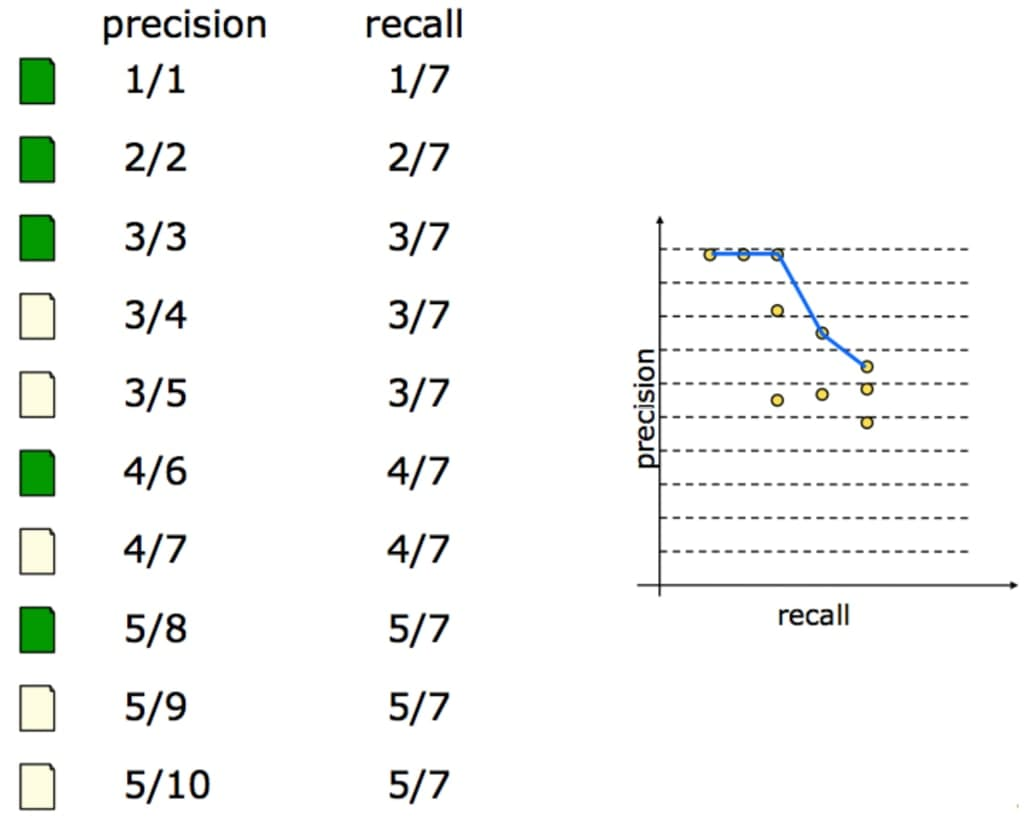
\includegraphics[height=0.7\textheight]{img/ranking_precision_recall.jpg}
\end{center}
С полнотой проблема: как правило, мы не знаем, сколько всего релевантных документов в индексе (базе).
\end{frame}

\begin{frame}{DCG}
    \begin{itemize}
        \item $\text{DCG}_K = l_1 + \sum_{i=2}^K\frac{l_i}{\log_2(i+1)}$: Discount Cumulative Gain. Чем дальше находится релевантный документ от топа, тем больше штраф.
        \item $\text{IDCG}_K$ (Ideal DCG): DCG для идеального ранжирования $K$ документов.
        \item $\text{nDCG} = \frac{\text{DCG}_K}{\text{IDCG}_K}$.
    \end{itemize}
\end{frame}

\begin{frame}{pFound}
\begin{itemize}
    \item Предполагаем, что пользователь просматривает документы подряд сверху вниз. $pBreak$ -- вероятность устать и прекратить поиск (не зависит от позиции и релевантности документа).
    \item $pRel(l_i) \in [0, 1)$ -- вероятность, что пользователь найдёт ответ в документе с релевантностью $l_i$.
    \item $pLook(l_i) = pLook(l_{i-1})(1-pRel(l_{i-1}))(1-pBreak)$ – вероятность дойти до $i$-го документа.
    \item $pFound@K = \sum_{i=1}^K pLook(l_i) \cdot pRel(l_i)$ – вероятность найти ответ на $K$ первых документах.
\end{itemize}
\end{frame}
\end{document}
